% \setchapterpreamble[u]{\margintoc}
\chapter{Term positions and stacks}
\labch{coq-positions}

As we will see in \nrefch{coq-reduction} and \nrefch{coq-conversion}, when
manipulating terms we sometimes have to go deep withing subterms.
Positions point you to a specific subterm of a term while stacks operate as
some sort of terms with a hole or equivalently some evaluation environments.

\section{Positions}

In a general setting, positions in trees are given by sequences of choices or
directions. The empty sequence corresponds to the root of the tree, and at each
branching you have to say which branch you want to take.

\marginnote[1cm]{
  Sequences such as \(0.1.0\) are read from left to right, and correspond to
  directions starting from the root.
  In black is the subtree as the given position.
}
\begin{figure}[hb]
  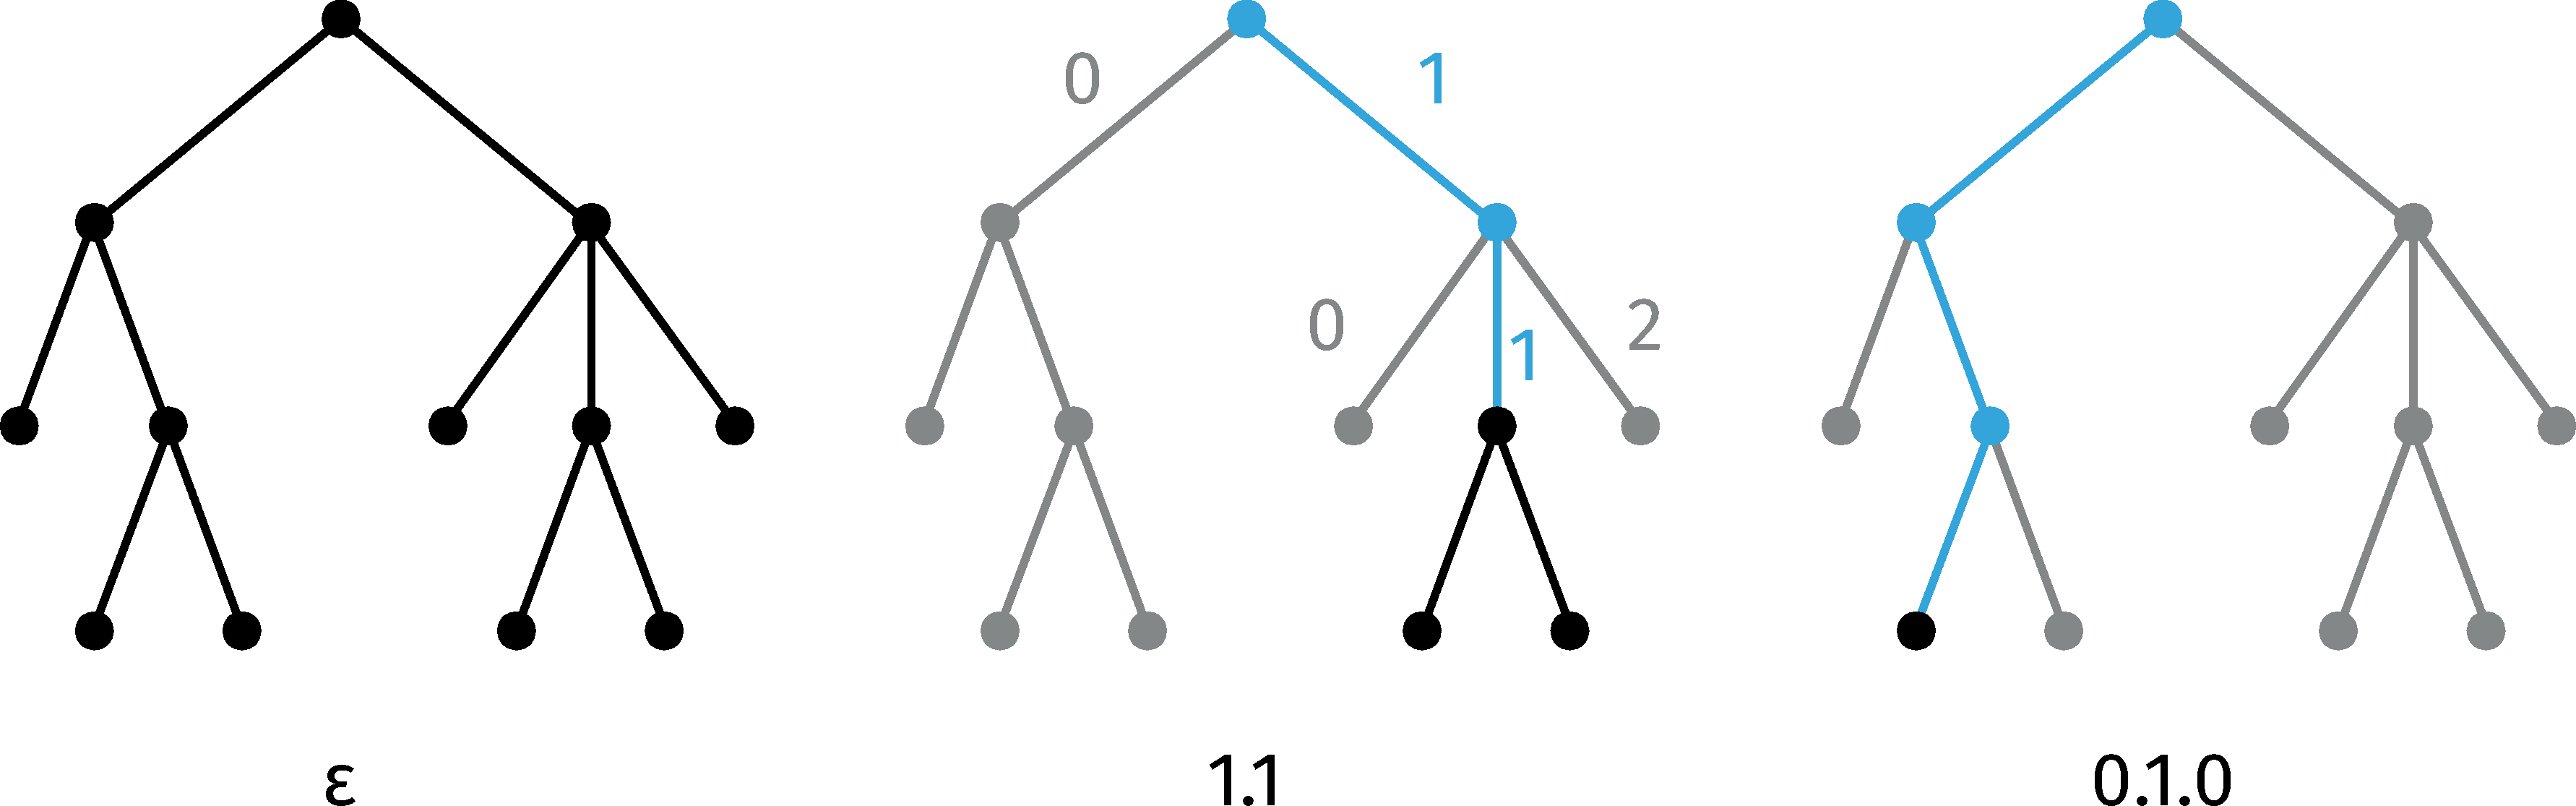
\includegraphics[width=0.9\textwidth]{tree-position.pdf}
\end{figure}

Now, terms are a special kind of tree so we can do something similar.
There are many ways to represent positions: for instance in the example above
the position \(0.3\) does not correspond to anything, so is it still considered
a position, only an \emph{invalid} one? Or should all expressable positions
be valid?

My approach is a bit in between, I constrain the syntax of choices a bit more
than this, but they are not necessarily valid.
Basically choices are defined inductively, with several constructors for each
of the constructs of the syntax: for instance, applications will have two
corresponding choices, one for the applicant, one for the argument.
\marginnote[1cm]{
  \mintinline{coq}{app_l} corresponds to going left under an application
  while \mintinline{coq}{app_r} corresponds to going right.
}
\begin{minted}{coq}
Inductive choice :=
| app_l
| app_r
| case_p
| case_c
| case_brs (n : nat)
| proj_c
| fix_mfix_ty (n : nat)
| fix_mfix_bd (n : nat)
| lam_ty
| lam_tm
| prod_l
| prod_r
| let_bd
| let_ty
| let_in.
\end{minted}

A position is just a list of choices.
\begin{minted}{coq}
Definition position := list choice.
\end{minted}

Now as I already said, these are not necessarily valid positions, for this
we define a function which verifies if a given position is valid in a given
term.
\marginnote[1cm]{
  It should not feel too surprising, the empty position is always valid,
  and otherwise, the head choice should match the structure of the term.
  There are some trickier cases for pattern-matching and fixed-points because
  they involve lists of terms but it is still pretty natural.
}
\begin{minted}{coq}
Fixpoint validpos t (p : position) {struct p} :=
  match p with
  | [] => true
  | c :: p =>
    match c, t with
    | app_l, tApp u v => validpos u p
    | app_r, tApp u v => validpos v p
    | case_p, tCase indn pr c brs => validpos pr p
    | case_c, tCase indn pr c brs => validpos c p
    | case_brs n, tCase indn pr c brs =>
        match nth_error brs n with
        | Some (_, br) => validpos br p
        | None => false
        end
    | proj_c, tProj pr c => validpos c p
    | fix_mfix_ty n, tFix mfix idx =>
        match nth_error mfix n with
        | Some d => validpos d.(dtype) p
        | None => false
        end
    | fix_mfix_bd n, tFix mfix idx =>
        match nth_error mfix n with
        | Some d => validpos d.(dbody) p
        | None => false
        end
    | lam_ty, tLambda na A t => validpos A p
    | lam_tm, tLambda na A t => validpos t p
    | prod_l, tProd na A B => validpos A p
    | prod_r, tProd na A B => validpos B p
    | let_bd, tLetIn na b B t => validpos b p
    | let_ty, tLetIn na b B t => validpos B p
    | let_in, tLetIn na b B t => validpos t p
    | _, _ => false
    end
  end.
\end{minted}
This function might serve as a specification for the positions.

Finally we can define a type of valid positions in a term using a subset type.
\begin{minted}{coq}
Definition pos (t : term) :=
  { p : position | validpos t p = true }.
\end{minted}

For instance \mintinline{coq}{[ app_l ; let_in ]} is valid position in term
\begin{minted}{coq}
  tApp (tLetIn na b B t) u
\end{minted}
which represents the term \mintinline{coq}{(let na := b : B in t) u}
and points to subterm \mintinline{coq}{t}.

We can also define a function to access the subterm at a given position.
\begin{minted}{coq}
Fixpoint atpos t (p : position) {struct p} : term :=
  match p with
  | [] => t
  | c :: p =>
    match c, t with
    | app_l, tApp u v => atpos u p
    | app_r, tApp u v => atpos v p
    | case_p, tCase indn pr c brs => atpos pr p
    | case_c, tCase indn pr c brs => atpos c p
    | case_brs n, tCase indn pr c brs =>
        match nth_error brs n with
        | Some (_, br) => atpos br p
        | None => tRel 0
        end
    | proj_c, tProj pr c => atpos c p
    | fix_mfix_ty n, tFix mfix idx =>
        match nth_error mfix n with
        | Some d => atpos d.(dtype) p
        | None => tRel 0
        end
    | fix_mfix_bd n, tFix mfix idx =>
        match nth_error mfix n with
        | Some d => atpos d.(dbody) p
        | None => tRel 0
        end
    | lam_ty, tLambda na A t => atpos A p
    | lam_tm, tLambda na A t => atpos t p
    | prod_l, tProd na A B => atpos A p
    | prod_r, tProd na A B => atpos B p
    | let_bd, tLetIn na b B t => atpos b p
    | let_ty, tLetIn na b B t => atpos B p
    | let_in, tLetIn na b B t => atpos t p
    | _, _ => tRel 0
    end
  end.
\end{minted}
\marginnote[-2.5cm]{
  The \mintinline{coq}{tRel 0} case is in an impossible branch when the position
  is valid, but for simplicity, the function is defined for any position.
  Otherwise we would have to carry the proof that it is valid everywhere.
}

Positions let you go deep inside a term, forgetting about its surrounding;
surrounding which can be recorded using stacks.

\section{Stacks}

My use of the term \emph{stack} might be an abuse as it is probably a
generalisation of it and might be better called an evaluation environment
or context; I will stick to \emph{stack} anyway.
The main reason behind the name is that it is not presented as a term with a hole
but rather as a succession of terms with a hole that stack on top of each other.

If you take the following example,
\[
  \stack{f\ \stack{\stack{(\lambda x. \stack{t})}\ u}}
\]
you are considering term \(t\) against the stack
\[
  \stack{f\ \stack{\stack{(\lambda x. \shole)}\ u}}
\]

It can be decomposed into
\marginnote[1cm]{
  \(\varepsilon\) represents the empty stack.
}
\[
  \stack{\lambda x. \shole} :: \stack{\shole\ u} :: \stack{f\ \shole}
  :: \varepsilon
\]
meaning that the term will first be put under an abstraction, the result of this
applied to \(u\) and the whole given as an argument to \(f\).
This notion will prove particularly useful when considering the reduction
machine in \nrefch{coq-reduction}. Indeed the stack is a way to remember the
surrounding term when focusing on a subterm. Once it has reached a normal form,
we can use the stack as a \emph{continuation}.

You can see the process step by step in the following example.
\marginnote[2cm]{
  I use \(\red_\beta\) to denote the cases where a \emph{real} reduction
  happens and the focused term (a \(\lambda\)-abstraction) consumes its
  argument; the other cases are \emph{focusing}, \ie pushing some term with
  hole on the stack.
}
\[
  \begin{array}{lc}
    \stack{
      (
        (\lambda x.\ x\ u)\
        (\lambda y.\ y)
      ) \ v
    } & \red \\[0.2cm]
    \stack{
      \stack{(
        (\lambda x.\ x\ u)\
        (\lambda y.\ y)
      )} \ v
    } & \red \\[0.3cm]
    \stack{
      \stack{(
        \stack{(\lambda x.\ x\ u)}\
        (\lambda y.\ y)
      )} \ v
    } & \red_\beta \\[0.4cm]
    \stack{
      \stack{(
        (\lambda y.\ y)\ u
      )} \ v
    } & \red \\[0.3cm]
    \stack{
      \stack{(
        \stack{(\lambda y.\ y)}\ u
      )} \ v
    } & \red_\beta \\[0.4cm]
    \stack{
      \stack{u} \ v
    }
  \end{array}
\]

\marginnote{
  In the formalism above, \(\vscmd{t}{\stack{\shole\ u} :: \varepsilon}\)
  corresponds to \(\stack{\stack{t}\ u}\). I am simply now making explicit
  the separation between the focused term and the stack.
}
The intesting bit is that the focused term still interacts with the stack.
To see clearer we can use the notation \(\vscmd{t}{\pi}\) representing
term \(t\) \emph{against} stack \(\pi\). From this we can write the following
reduction rules that together correspond to \(\beta\)-reduction.

\marginnote[0.5cm]{
  \(\beta\)-reduction now happens in two steps:
  \(
    \vscmd{(\lambda x.\ t)\ u}{\pi} \red
    \vscmd{\lambda x.\ t}{\stack{\shole\ u} :: \pi} \red
    \vscmd{t[x \sto u]}{\pi}
  \)
}
\[
  \begin{array}{lcl}
    \vscmd{u \ v}{\pi} &\red& \vscmd{u}{\stack{\shole\ v} :: \pi} \\
    \vscmd{\lambda x.\ t}{\stack{\shole\ u} :: \pi}
    &\red& \vscmd{t[x \sto u]}{\pi}
  \end{array}
\]

In \Coq I define stacks as follows.
\begin{minted}{coq}
Inductive stack : Type :=
| Empty
| App (t : term) (π : stack)
| Fix (f : mfixpoint term) (n : nat) (args : list term)
      (π : stack)
| Fix_mfix_ty (na : name) (bo : term) (ra : nat)
              (mfix1 mfix2 : mfixpoint term) (id : nat)
              (π : stack)
| Fix_mfix_bd (na : name) (ty : term) (ra : nat)
              (mfix1 mfix2 : mfixpoint term) (id : nat)
              (π : stack)
| CoFix (f : mfixpoint term) (n : nat) (args : list term)
        (π : stack)
| Case_p (indn : inductive * nat) (c : term)
         (brs : list (nat * term)) (π : stack)
| Case (indn : inductive * nat) (p : term)
       (brs : list (nat * term)) (π : stack)
| Case_brs (indn : inductive * nat) (p c : term) (m : nat)
           (brs1 brs2 : list (nat * term)) (π : stack)
| Proj (p : projection) (π : stack)
| Prod_l (na : name) (B : term) (π : stack)
| Prod_r (na : name) (A : term) (π : stack)
| Lambda_ty (na : name) (b : term) (π : stack)
| Lambda_tm (na : name) (A : term) (π : stack)
| LetIn_bd (na : name) (B t : term) (π : stack)
| LetIn_ty (na : name) (b t : term) (π : stack)
| LetIn_in (na : name) (b B : term) (π : stack)
| coApp (t : term) (π : stack).

Notation "'ε'" := (Empty).
\end{minted}

\section{Positions induced by stacks}

The reason I present stacks and positions together is because they are related.
If you consider the term \(t\) against some stack \(\pi\) as one term, there
exists a position in that term that points to \(t\).
For instance if you consider
\[
  \stack{u\ \stack{\stack{t}\ v}}
\]
then the position that first chooses the right-hand term of the top-level
application and then the left-hand term will indeed point to \(t\).
In \Coq syntax as earlier this would be
\begin{minted}{coq}
[ app_r ; app_l ]
\end{minted}

In fact the position can be computed from the stack itself, regardless of the
term we want to plug in. In the example above, the stack is
\[
  \stack{\shole\ v} :: \stack{u\ \shole} :: \varepsilon
\]
We read it from right to left\sidenote{This is because the leftmost term with
hole corresponds to the innermost element in the resulting term.} to reconstruct
the position and simply give the position of the hole.

\begin{minted}{coq}
Fixpoint stack_position π : position :=
  match π with
  | ε => []
  | App u ρ => stack_position ρ ++ [ app_l ]
  | Fix f n args ρ => stack_position ρ ++ [ app_r ]
  | Fix_mfix_ty na bo ra mfix1 mfix2 idx ρ =>
      stack_position ρ ++ [ fix_mfix_ty #|mfix1| ]
  | Fix_mfix_bd na ty ra mfix1 mfix2 idx ρ =>
      stack_position ρ ++ [ fix_mfix_bd #|mfix1| ]
  | CoFix f n args ρ => stack_position ρ ++ [ app_r ]
  | Case_p indn c brs ρ => stack_position ρ ++ [ case_p ]
  | Case indn pred brs ρ => stack_position ρ ++ [ case_c ]
  | Case_brs indn pred c m brs1 brs2 ρ =>
      stack_position ρ ++ [ case_brs #|brs1| ]
  | Proj pr ρ => stack_position ρ ++ [ proj_c ]
  | Prod_l na B ρ => stack_position ρ ++ [ prod_l ]
  | Prod_r na A ρ => stack_position ρ ++ [ prod_r ]
  | Lambda_ty na u ρ => stack_position ρ ++ [ lam_ty ]
  | Lambda_tm na A ρ => stack_position ρ ++ [ lam_tm ]
  | LetIn_bd na B u ρ => stack_position ρ ++ [ let_bd ]
  | LetIn_ty na b u ρ => stack_position ρ ++ [ let_ty ]
  | LetIn_in na b B ρ => stack_position ρ ++ [ let_in ]
  | coApp u ρ => stack_position ρ ++ [ app_r ]
  end.
\end{minted}

As I said multiple times, we will use stacks for reduction machines, to show the
termination of such machines it is nice to have an order on stacks. This order
will be achieved by going from stacks to positions.

\section{Ordering positions}

If you consider the valid positions in a given term (\ie expressions of type
\mintinline{coq}{pos t} for some \mintinline{coq}{t}) there exists a
well-founded order on them. There are actually several due to some degree of
liberty as we shall see.

Since positions are defined as lists, the natural order on them would the
structural one which says that any (strict) prefix of a position is smaller.
This order is not really of interest to us because it would correspond to
\emph{unfocusing}.
Conversely, by extending a position with a new choice you are going deeper into
the term, something which you cannot do indefinitely, you are bound to reach a
leaf at some (finite) point.

If you think about it dually, I am merely explaining that the structural order on
terms is well-founded, so why bother?
The interesting part is that the order on positions can be more flexible than
the subterm relation in that it allows us to compare `going left' with
`going right'.
Say you have the application \(t \coloneqq u\ v\), both \(u\) and \(v\) are
subterms of \(t\) but there is no way to relate the two of them reliably and
have \(v\) \emph{always} smaller than \(u\) because \(u\) and \(v\) can be
arbitrary.
If instead we were to consider positions in \(t\) we would have the empty one
corresponding to \(t\) itself, \mintinline{coq}{[ app_l ]} corresponding to
\(u\) and \mintinline{coq}{[ app_r ]} for \(v\). This means we abstract over the
content of both \(u\) and \(v\). The positions can thus be ordered as follows:
\begin{minted}{coq}
[ app_r ] < [ app_l ] < []
\end{minted}

I am going to explain why this is desirable in \nrefch{coq-reduction}.

In \Coq, the definition of the order is done in two steps: first an order on
raw positions, from which we then derive an order on valid positions.
\marginnote[4.8cm]{
  The \mintinline{coq}{(` p)} notation corresponds to the first projection of
  a subset type.
}
\begin{minted}{coq}
Inductive positionR : position -> position -> Prop :=
| positionR_app_lr p q :
    positionR (app_r :: p) (app_l :: q)

| positionR_deep c p q :
    positionR p q ->
    positionR (c :: p) (c :: q)

| positionR_root c p :
    positionR (c :: p) [].

Definition posR {t} (p q : pos t) : Prop :=
  positionR (` p) (` q).
\end{minted}

While the first order is not well-founded, the second one is, as crystallised
by the following lemma.
\begin{minted}{coq}
Lemma posR_Acc :
  forall t p, Acc (@posR t) p.
\end{minted}